\chapter{Experiments} \label{chapter:experiments}

In this chapter, we evaluate how effective our learned cost function is, which is described below, where $D$ is the number of features, $A$ is the set of actions and the resulting value of $\mathbf{x}$ after the interventions is $\mathbf{x}^{\text{PCF}}$.

\begin{align} \label{eq:cost_function_experiments}
	\cost(A, \beta_k, \mathcal{F}) & = \sum_{i=1}^D \delta_i \beta_{ki}^2 \\ \nonumber
	A & = \big\{(\mathbf{S}, \text{do} \{\mathbf{x}_i:=\mathbf{x}_i + \boldsymbol{\delta}_i\}_{i=1, \ldots, D})\big\} \\ \nonumber
	\mathbf{x}^{\text{PCF}} & = \mathbb{I}_{i \in I} \boldsymbol{\delta}_i + \bigg( \mathbf{x}_i + f_i(\textbf{pa}^{\text{PCF}}_i) - f_i(\textbf{pa}_i) \bigg)
\end{align}

\section{End-to-End Methodology}

The end-to-end methodology for generating recourse with a learned cost is shown in Figure \ref{fig:workflow}, and more details on each of the steps in the methodology are described below.

\begin{figure}[!htb]
	\centering
	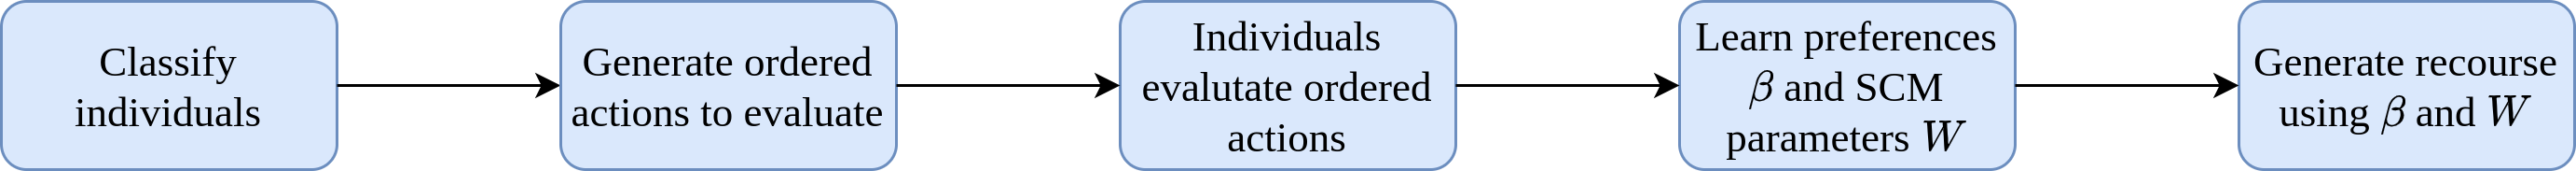
\includegraphics[width=\linewidth]{images/draw.io/workflow.png}
	\caption{End-to-End Methodology}
	\label{fig:workflow}
\end{figure}

\begin{enumerate}
	\item \textbf{Classify individuals}. Individuals with features $\mathbf{X}$ are assessed by a classifier and are classified either positively (e.g., loan approved, admission acceptance) or negatively (e.g., loan rejected, admission rejected). In this thesis, logistic regression has been used, largely for simplicity. However, as an augmented Lagrangian gradient descent optimisation is used to generate recourse (see section \ref{section:generating_recourse}), any differentiable classifier could be used instead of logistic regression.
	
	\item \textbf{Generate ordered actions to evaluate}. We randomly generate actions for each negatively classified individual and associated randomly generated orderings. This is another area for future work, where an online or Bayesian approach could be used to generate recourse actions to maximise information gain, such as the approach used in \textcite{detoniPersonalizedAlgorithmicRecourse2023}.
	
	\item \textbf{Users evaluate ordered actions}. Using the cost function described in equation \ref{eq:cost_function_experiments} with noisy user preferences $\tilde{\beta_k}$ and noisy SCM $\tilde{\mathcal{F}}$, users evaluate which of the ordered actions they are presented with they prefer. 
	
	\item \textbf{Learn preferences $\hat{\beta_k}$ and SCM approximation parameters $\hat{W}$}. The model deployer then learns user preferences $\hat{\beta_k}$ and a linear approximation of the true SCM $\hat{W}$ using the optimisation presented in section \ref{section:cost_learning_formulation}.
	
	\item \textbf{Generate recourse using $\hat{\beta_k}$ and $\hat{W}$}. The model deployer then generates recourse $\mathbf{X}^*$ for the negatively classified users.
	
\end{enumerate}
\bigskip


\section{Synthetic Data}

We create synthetic SCMs, from which we sample our data $\mathbf{X}$. We simulate two different SCMs, the first being a linear SCM and the second a non-linear SCM.

\subsection{Linear SCM} \label{section:linear_scm}

Shown below are the structural equations of the linear SCM $\mathcal{M}_{\text{LIN}}$ as well as the associated causal graph, where $\sigma$ is the sigmoid function.

\begin{align} \label{eq:linear_scm_structural_equations}
	x_1 & = u_1 & u_1 \sim N(0,1) \\ \nonumber
	x_2 & = u_2 + 0.5x_1 & u_2 \sim N(0,1) \\ \nonumber
	x_3 & = u_3 + 0.2x_1 + 0.3x_2 & u_3 \sim N(0,0.5) \\ \nonumber
	y   & \sim \text{Bernoulli}(\sigma(0.1x_1 + 0.2x_2 + 0.3x_3))
\end{align}

\begin{figure}[!htb]
	\centering
	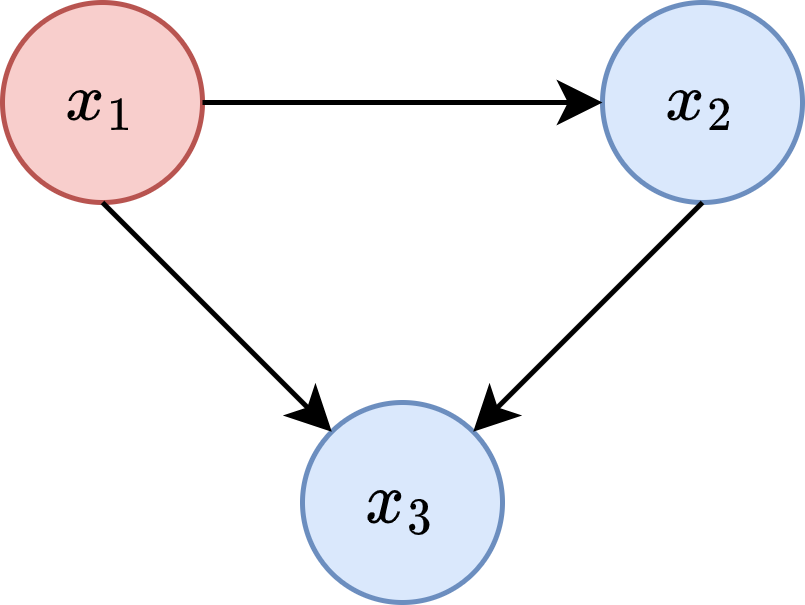
\includegraphics[width=0.4\linewidth]{images/draw.io/toy_scm.png}
	\caption{Linear SCM $\mathcal{M}_{\text{LIN}}$}
	\label{fig:simple_scm}
\end{figure}

\subsection{Non-Linear SCM}

Shown below are the structural equations of the non-linear SCM $\mathcal{M}_{\text{NL}}$ as well as the associated causal graph, where $\sigma$ is the sigmoid function.

\begin{align}
	x_1 & = u_1 & u_1 \sim N(0,1) \\ \nonumber
	x_2 & = u_2 - \frac{2}{1 + x_1^2} & u_2 \sim N(0,1) \\ \nonumber
	x_3 & = u_3 + 0.1x_1 + 0.3x_1x_2 & u_3 \sim N(0,0.5) \\ \nonumber
	x_4 & = u_4 + 0.6x_1 - 0.2x_2x_3 & u_4 \sim N(0,0,5) \\ \nonumber
	x_5 & = u_5 + 0.8x_4 & u_5 \sim N(0,0.5) \\ \nonumber
	y   & \sim \text{Bernoulli}(\sigma(0.1x_1 + 0.2x_2 + 0.3x_3 + 0.4x_4 + 0.5x_5))
\end{align}

\begin{figure}[!htb]
	\centering
	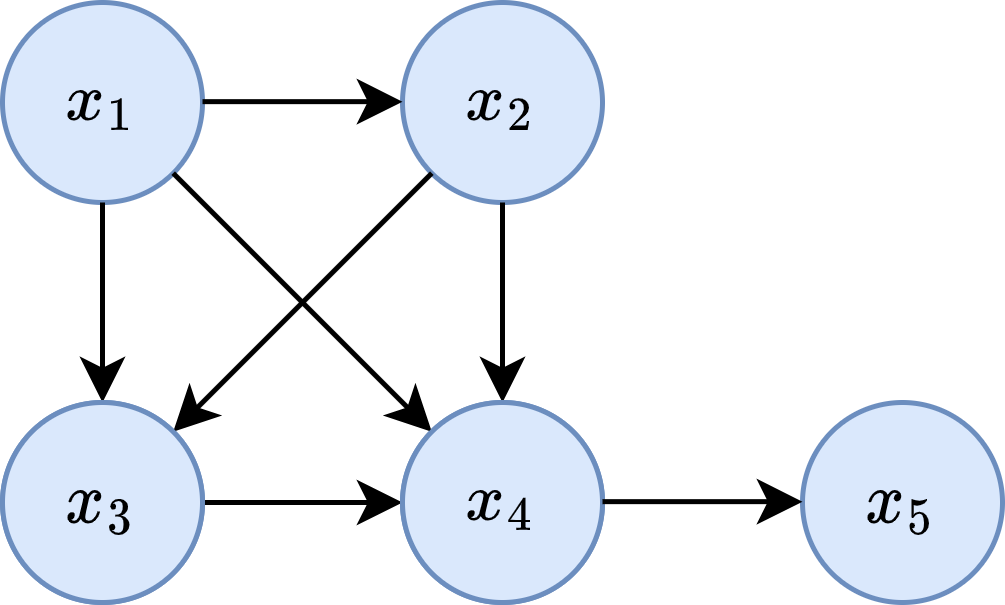
\includegraphics[width=0.5\linewidth]{images/draw.io/non_linear_scm.png}
	\caption{Non-Linear SCM $\mathcal{M}_{\text{NL}}$}
	\label{fig:non_linear_scm}
\end{figure}


\section{Evaluation Metrics} 

We will use two metrics to assess the performance of our methodology.\\

We refer to the first as the \textit{average increase in cost}. This is the percentage increase of the average cost (calculated using the ground truth $\beta$ and true SCM) of recourse generated using a learned $\hat{\beta}$ and approximation of the SCM $\hat{W}$ compared to the average cost (calculated using the ground truth $\beta$ and true SCM) of recourse generated using the ground truth $\beta$ and true SCM. We use this metric for several reasons.\\

\begin{enumerate}
	\item Costs are calculated using the ground truth user preferences $\beta$ and the true SCM, meaning that we are measuring the true cost of recourse to each individual, as opposed to estimated cost using the learned $\hat{\beta}$ and the learned approximation of the SCM $\hat{W}$.
	
	\item The cost of recourse is a rather abstract concept, especially when we define it numerically. It is not particularly intuitive to report that the cost of increasing your income by £10,000 and your savings by £5,000 is 3.14 units. However, it may be more intuitive to report that the recourse we have computed is 31.4\% more costly than if we had used the ground truth user preferences and the true SCM.
\end{enumerate}

\bigskip

The second metric, which we refer to as the \textit{average $L_2$ norm}, measures how well we have recovered user preferences $\beta$. Firstly, we calculate the average $L_2$ norm of $\hat{\beta}_k - \hat{\beta}_k$. For each user, we calculate the L2 norm between the difference between their true and predicted user preferences. This gives a measure of, on average, how well we have recovered the user preferences. \\

\section{Results}

In this section, we present the results of our methodology on the linear SCM and the non-linear SCM. We start in the case where all individuals have homogeneous preferences $\beta$ and then relax this assumption to a more realistic case where individuals have different preferences $\beta_k$. In each experiment, we show the effect of different numbers of paired comparisons the individuals are asked. \\

As discussed in section \ref{section:noisy_responses}, we also assume that individuals have \textit{noisy} local knowledge of the SCM and evaluate their preferences with some noise. For both of these sources of noise, we assume that the noise is drawn from the distribution $N(0, \sigma^2)$. In each experiment, we show the increasing noise, by varying the standard deviation parameter $\sigma$. \\

As a baseline, we compare our results to the naive case where we do not know either user preferences or the true SCM. Therefore, user preferences are assumed to be uniformly distributed (for 3 variables, $\beta = [1/3, 1/3, 1/3]$) and as we do not know the true SCM, the linear approximation of the SCM $\hat{W}$ is simply the identity matrix. This corresponds to assuming there are no causal relationships between features.

\subsection{Homogeneous Preferences over Feature Mutability}

In the linear SCM where individuals have homogeneous preferences, we set individuals' preferences over feature mutability as $\beta = [0.7, 0.2, 0.1]$. The results are shown in Figure \ref{fig:simple_single_beta}, where the learned cost function leads to a very similar cost of recourse when using the ground truth preferences and true SCM and successfully recovers the users' preferences.

\begin{figure}[!htb]
	\centering
	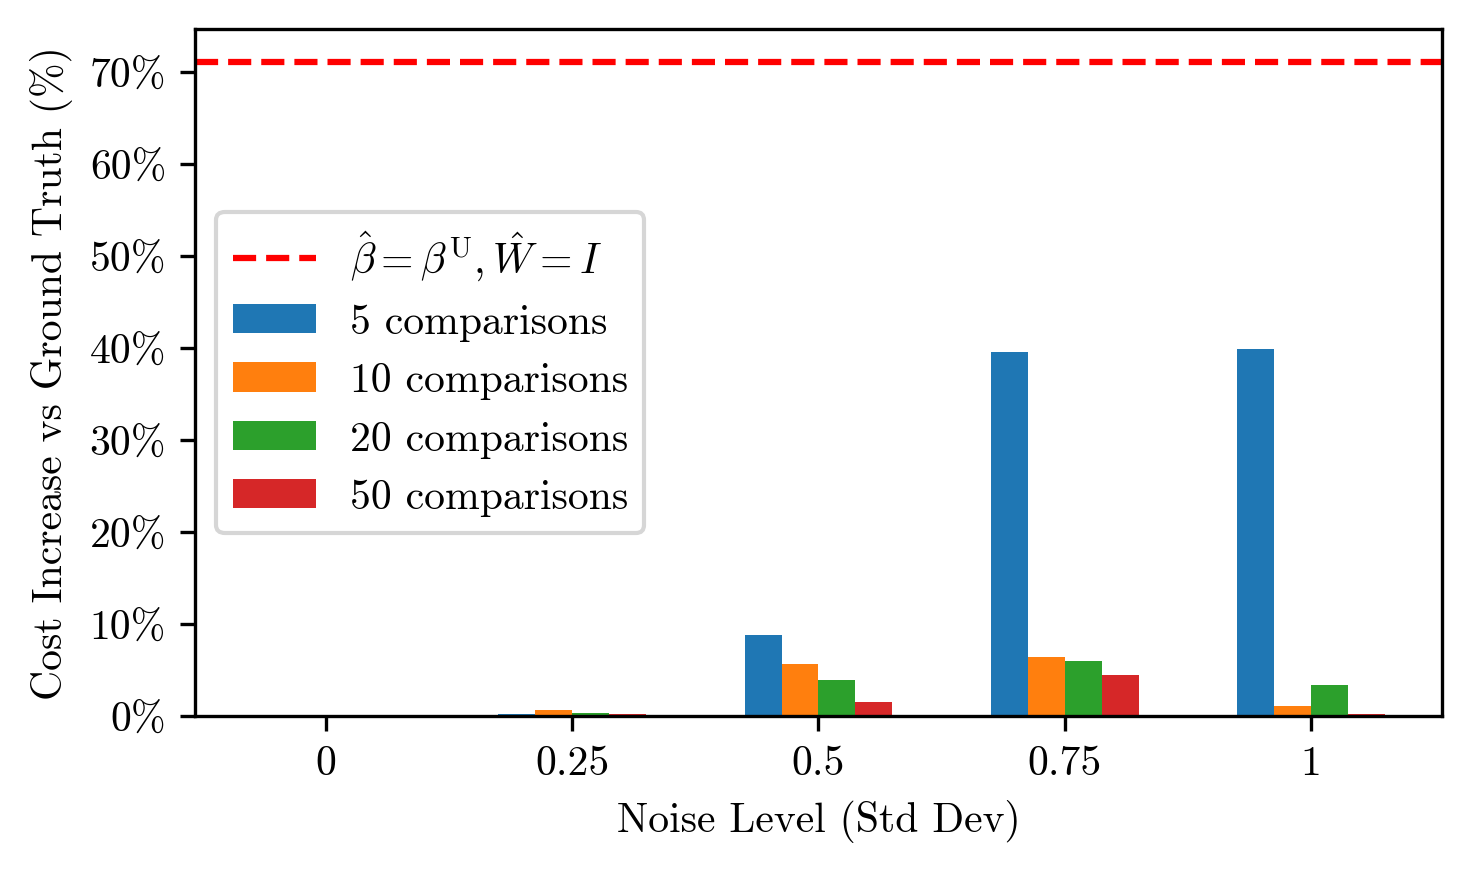
\includegraphics[width=0.75\linewidth]{../plots/simple_single_beta.png}
	\caption{Increase in average cost compared to ground truth for different noise levels using a linear SCM and a single $\beta$ for all individuals.}
	\label{fig:simple_single_beta}
\end{figure}

In addition to recovering the users' preferences, we also successfully recover the parameters of the true SCM. Using the structural equations of the linear SCM defined in equation \ref{eq:linear_scm_structural_equations}, we can express the true parameters as a weighted adjacency matrix, which is shown below.

\begin{equation}
	W_{\text{TRUE}} = 
	\begin{bmatrix}
		1 & 0.5 & 0.35 \\
		0 & 1 & 0.3 \\
		0 & 0 & 1
	\end{bmatrix}
\end{equation}

In the noiseless setting, we learn the below parameters of the approximation of the SCM - showing a successful recovery of the parameters of the SCM. Given that this is a linear approximation of a linear SCM, it is unsurprising that we fully recover the parameters.

\begin{align}
	& \hat{W}_5 =
	\begin{bmatrix}
		1 & 0.49 & 0.34 \\
		-0.008 & 1 & 0.31 \\
		-0.0002 & -0.02 & 1
	\end{bmatrix}
	\quad
	& \hat{W}_{10} =
	\begin{bmatrix}
		1 & 0.49 & 0.33 \\
		-0.002 & 1 & 0.29 \\
		-0.0005 & -0.01 & 1
	\end{bmatrix} \\ \nonumber
	& \hat{W}_{20} =
	\begin{bmatrix}
		1 & 0.50 & 0.35 \\
		0.001 & 1 & 0.30 \\
		0.002 & -0.003 & 1
	\end{bmatrix}
	& \hat{W}_{50} =
	\begin{bmatrix}
		1 & 0.50 & 0.35 \\
		-0.0003 & 1 & 0.29 \\
		0.0009 & 0.0004 & 1
	\end{bmatrix}
\end{align}


We also repeat the same experiment for the non-linear SCM. For this SCM, with five variables, we set user preferences at $\beta = [0.05, 0.05, 0.6, 0.15, 0.15]$. The results are shown in Figure \ref{fig:nonlinear_single_beta}. Whilst the user preferences are still well recovered, the cost of recourse now becomes significantly greater (when compared to recourse generated using the ground truth preferences and true SCM). This is caused by the fact that we are modelling a non-linear SCM with a linear approximation. Nonetheless, the cost of recourse is still significantly lower than the naive baseline of uniform preferences and assumes no causal effects.

\begin{figure}[!htb]
	\centering
	\includegraphics[width=0.75\linewidth]{../plots/nonlinear_single_beta.png}
	\caption{Increase in average cost compared to ground truth for different noise levels using a non-linear SCM and a single $\beta$ for all individuals.}
	\label{fig:nonlinear_single_beta}
\end{figure}

\subsection{Heterogeneous Preferences over Feature Mutability}

Now, we relax the (restrictive) assumption that individuals have homogeneous preferences and assume that each individual $k$ has their own preferences over feature mutability $\beta_k$. Many users will likely have similar preferences - for example, increasing the level of education is likely much more difficult than increasing savings for many individuals. Therefore, the true user preferences are defined as $\beta_k = [0.7, 0.2, 0.1] + u$ where $u \sim \text{Gamma}(0.05, 1)$ and $u \in \mathbb{R}^3$. Nonetheless, in this setting, an individualised $\hat{\beta}_k$ is learned for each individual.\\

The results are shown below in Figure \ref{fig:simple} for the linear SCM. Compared to Figure \ref{fig:simple_single_beta}, we see significantly worse recovery of the true user preferences, which feeds into the significantly increased cost of recourse. However, recovery of the parameters of the true SCM is still successful, as shown below where the (noiseless) learned parameters $\hat{W}$ are still very similar to the parameters of the true SCM.

\begin{align}
	& \hat{W}_5 =
	\begin{bmatrix}
		1 & 0.54 & 0.31 \\
		-0.01 & 1 & 0.29 \\
		0.03 & 0.01 & 1
	\end{bmatrix}
	\quad
	& \hat{W}_{10} =
	\begin{bmatrix}
		1 & 0.54 & 0.34 \\
		0.005 & 1 & 0.33 \\
		0.0005 & -0.02 & 1
	\end{bmatrix} \\ \nonumber
	& \hat{W}_{20} =
	\begin{bmatrix}
		1 & 0.52 & 0.36 \\
		0.001 & 1 & 0.30 \\
		-0.002 & -0.007 & 1
	\end{bmatrix}
	& \hat{W}_{50} =
	\begin{bmatrix}
		1 & 0.51 & 0.35 \\
		0.0005 & 1 & 0.30 \\
		0.0006 & -0.004 & 1
	\end{bmatrix}
\end{align}



\begin{figure}[!htb]
	\centering
	\includegraphics[width=0.75\linewidth]{../plots/simple.png}
	\caption{Increase in average cost compared to ground truth for different noise levels using a linear SCM and a different $\beta_k$ for each individual.}
	\label{fig:simple}
\end{figure}

The same experiment is repeated for the non-linear SCM. The user preferences are again assumed to be similar for most individuals and are defined as $\beta_k = [0.05, 0.05, 0.6, 0.15, 0.15] + u$ where $u \sim \text{Gamma}(0.05, 1)$ and $u \in \mathbb{R}^5$. The results are shown below in Figure \ref{fig:nonlinear}. Here the performance of the learned cost function for 5 and 10 comparisons is roughly in line with the naive baseline of uniform preferences and no causal effects, and it is only when we increase the number of comparisons to 20 that we see an improved estimation of the user preferences and lower cost of recourse.


\begin{figure}[!htb]
	\centering
	\includegraphics[width=0.75\linewidth]{../plots/nonlinear.png}
	\caption{Increase in average cost compared to ground truth for different noise levels using a non-linear SCM and a different $\beta_k$ for each individual.}
	\label{fig:nonlinear}
\end{figure}


\section{Discussion} \label{section:discussion}

Our results show that, in simpler settings with homogeneous preferences and a linear SCM, our methodology to learn feature mutability and causal relations results in \textit{significantly} less costly recourse. Even with heterogeneous preferences and a linear SCM or homogeneous preferences and a non-linear SCM, there are significant advantages to learning from the individuals' revealed preferences. However, performance deteriorates as more complex settings are introduced. \\

A key reason for this decline in performance is that, without presenting the negatively classified individuals with a very large number of comparisons, the user preferences $\beta_k$ are not recovered effectively. In the current methodology, the paired comparisons which are presented to the users are selected randomly, as opposed to taking an approach similar to \textcite{detoniPersonalizedAlgorithmicRecourse2023}, which maximises the \textit{Expected Utility of Selection}. This is an area for further research, incorporating techniques to select paired comparisons to maximise information gain.\\

It is important to note that to properly evaluate the performance of any algorithmic recourse methodology, we would likely need to conduct a user study. In our synthetic data set-up, we designed SCMs which describe the world and assumed that individuals have \textit{local} knowledge of the SCM. We used these SCMs and our assumed cost function to simulate responses to paired comparisons and also to calculate the `true' cost of recourse. However, negatively classified individuals in the real world may have a very different cost function. Additionally, the true SCM that governs the real world could be highly complex and our linear approximation may perform poorly against the true SCM. We cannot truly compare how costly the recourse that we generate using our methodology is without having real negatively classified individuals evaluate how suitable the recourse we generate is.